\documentclass[12pt]{report}
\usepackage{graphicx,amssymb,amsmath,amsthm,ctable,booktabs,graphics}
\usepackage[colorlinks]{hyperref}
\usepackage[all]{hypcap} 
\usepackage{gensymb}
\usepackage{xcolor}
\usepackage{savetrees}
\usepackage{caption,subcaption}
\usepackage{multirow}
%\renewcommand{\familydefault}{\sfdefault}
\usepackage[english]{babel}
%\usepackage[T1]{fontenc}
%\usepackage{helvet}
\usepackage{multicol}
\usepackage[utf8x]{inputenc}

\renewcommand{\sectionautorefname}{\S} %for \autoref
\renewcommand{\subsectionautorefname}{\S} %for \autoref
\renewcommand{\subsubsectionautorefname}{\S} %for \autoref

\newcommand{\ty}[1]{\textcolor{teal}{\texttt{#1}}}
\begin{document}

\title{Gemini-South IFU Data Reduction User Manual}
\author{Elaine M. Snyder\\
Dept. of Physics \& Astronomy\\
University of North Carolina at Chapel Hill \\
\texttt{emsnyder@live.unc.edu}}
\date{February 22, 2016}
\maketitle

\hypersetup{linkcolor=magenta}
\tableofcontents
\begingroup
\let\clearpage\relax
\listoffigures
\listoftables
\endgroup

%\begin{multicols*}{2}

\chapter{Introduction}
Greetings, Gemini Multi-Object Spectrograph (GMOS) integral field unit (IFU) data reduction pipeline user! Before beginning your data reduction journey, it will be important to understand the structure of an IFU and the way the Gemini IFU data is stored in the fits files you'll be reducing. If you are familiar with this already, feel free to skip ahead. Most of this information can be found online on \url{https://www.gemini.edu}, but I've compiled it all here for easy reference and so that I may reference it in the context of the RESOLVE\footnote{\url{http://www.resolve.astro.unc.edu}} survey's instrument setups.

\section{What is an IFU and why would we want to use one?}
\label{ifu}
The basic idea of any spectrograph is that incoming light from an object goes through a slit, is dispersed by a grating/prism/grism, and then focused onto the CCD detector to create an image of the spectrum. Most of the time the slit is long and narrow ($\sim0.5-2''$ typically), and most astronomers would align it along a galaxy's major axis. This image will thus have spectral information in the x direction and spatial information in the y direction. The GMOS IFU is different in that instead of having one slit aligned along a galaxy's major axis, you will have multiple fibers that cover the entire galaxy. These fibers act as ``mini slits'', and each one will be dispersed and refocused onto the detector. This means you receive spectral information from all parts of the galaxy, not just where a single slit falls, and therefore are getting x, y, and wavelength at once. Thus, the main benefit of using an IFU is that it enables the 3D spatial analysis of the kinematics, metallicities, or whatever else you may want to derive from your spectra.

In the case of the GMOS IFU setups for RESOLVE observations, you will have either 750 or 1500 hexagonal fibers (depending on which setup was used) that cover an on-sky area of $5''\times3.5''$ or $7''\times5''$. The top-right portion of \autoref{figure:1} gives an example of the positions of the fibers over a galaxy. As the top left portion of \autoref{figure:1} shows, the GMOS IFU is designed in such a way that not all of the fibers are centered on the object -- either 250 or 500 of the fibers are positioned on a region of sky away from the target (but not too far away). This lets us observe separate spectra of the scattered light from our atmosphere, which can later be subtracted from the science spectra during data reduction. This ``sky level'' can be affected by moon illumination, clouds, etc. so it is important to be able to subtract any extra light there may be. Note that sometimes in online documents, the fibers may be called ``spaxels'', which is short for ``spectral pixels'' -- don't be confused by this hip IFU lingo.

\begin{figure}[h]
\centering
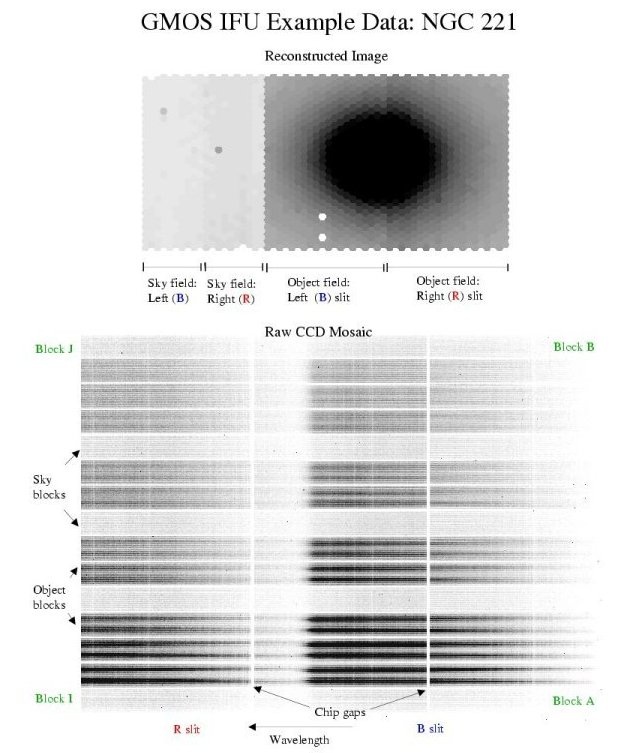
\includegraphics[width=0.8\textwidth]{fiber_examples.jpeg}
\caption[IFU Fibers and Data Format]{The top part of this image shows the IFU field of view over NGC221 (not a part of RESOLVE). The left portion of the image shows the sky spaxels, and the right portion shows the light of the galaxy. This is a 2D representation of the data we are getting -- the third dimension is in the wavelength direction, and the darkness over where the galaxy is from summing the light inside each spaxel there. The bottom portion of this image shows the raw fits data from the above galaxies.  \footnotesize{Image from \url{https://www.gemini.edu/sciops/instruments/gmos/spectroscopy/integral-field-spectroscopy/field-slit-mapping}}}
\label{figure:1}
\end{figure}

\section{Observing setups}
\label{setups}
As alluded to before, there are two main setups for RESOLVE's IFU observations. Similarly to our SOAR observations, there is a blue setup for absorption line galaxies and red setup for emission line galaxies. \autoref{table:1} highlights the main differences between the two setups. To determine which setup is best for which galaxy, we ideally like to use the SOAR broad spectrum as a guide. Seeing strong emission in the broad spectrum will point to the emission line setup on Gemini being best, while no emission will point to the absorption line setup being preferred. However, since there is not always a SOAR (or even an SDSS) spectrum available, we often rely on photometric colors as an indicator of whether emission or absorption is more likely.

Using the GMOS IFU is ideal for RESOLVE's purposes for two different reasons. In the red setup, our goal is to obtain velocity fields for RESOLVE's smallest emission line galaxies. Thus, the spatial information we receive from the IFU spectra is ideal for this purpose. On the other hand, for the blue setup, our goal is to derive velocity dispersions. The small, absorption line galaxies we target with the IFU in the blue setup are often quite faint, so instead of focusing on the spatial information the IFU gives, we sum all the spaxels out to the effective radius of the galaxy, thereby summing the light enough to derive accurate dispersion measurements. 

We estimate exposure times for both setups using the online Integration Time Calculators\footnote{\url{http://www.gemini.edu/node/10479}} (ITC) supplied by Gemini. We use an elliptical galaxy SED template for time estimates in the blue setup and adjust our exposure time calculations so that we may achieve a signal-to-noise ratio of 25 per \AA\ when we bin all the fibers out to the effective radius of the galaxy. We use a model H$\alpha$ line with estimates of the line flux and continuum flux density for time estimates in the red setup, and adjust our exposure times to achieve a centroiding accuracy of $\sim5.3$ km s$^{-1}$. For both setups, we bin our spectra by 2 in the spectral direction to increase the signal-to-noise as well.

We also use the ITC to select central wavelength positions that ensure our features of interest do not fall in a chip gap (see bottom of \autoref{figure:1}). We choose two different central wavelengths so that we can fill in the chip gaps as well when we sum the individual exposures -- this is sometimes referred to as ``spectral dithering''. The central wavelength positions selected for our setups are listed in \autoref{table:1}.

\begin{table}
\centering
\begin{tabular}[t]{|c|c|c|}
  \hline
quantity  & blue setup & red setup \\ \hline
wavelength range & 4200 -- 5600 \AA\ &  5500 -- 6900 \AA\ \\ 
used for & absorption line galaxies & emission line galaxies \\
central wavelengths & 4850, 4900 \AA\ & 6300, 6400 \AA\ \\
features of interest & H$\beta$, Mgb, Fe5270, Fe5335 & H$\alpha$, [NII], NaD \\ 
grating & B1200 & B600 \\ 
filter & none (open) & r-G0326 \\
slits & 1 slit & 2 slits \\ 
field of view & $3.5''\times5''$ & $5''\times7''$ \\ \hline
\end{tabular}
\caption[RESOLVE's Observation Setups]{Comparison of RESOLVE's red and blue observation setups for the Gemini-South IFU.}
\label{table:1}
\end{table}

\section{Observing patterns}
\label{patterns}
In 2-slit (aka red setup) mode, we oftentimes will tile the IFU field of view in order to cover the entire extent of the galaxy. The $5''\times7''$ field of view can either be tiled to $10''\times7''$ for larger, rounder galaxies or to  $5''\times14''$ for longer, skinnier galaxies. This doesn't make a large difference to the reduction routine, but there will be more science frames to reduce and more data cubes to stack at the end.

The basic observation sequence is different for each mode. See \autoref{table:2} for the basic order of the observations. Both will start with acquisition images to ensure the IFU field of view is centered on the galaxy. Then flats, arcs, and science frames are taken in each wavelength dither (denoted as $\lambda_{cen}$ in \autoref{table:2}) . For example, a flat, arc, science, and arc frame will be taken at one central wavelength, and then an arc, science, arc, flat frame will be taken at the other central wavelength. For the reduction, we will want to flat field and wavelength transform the science images using the arcs and flats taken in the same dither. Once the data cubes are made, we can then sum the data cubes, both spatially and spectrally.

\begin{table}
\centering
\begin{tabular}[t]{|c|c|c|c|c|}
  \hline
$\lambda_{cen}$ & blue setup & & red setup & $\lambda_{cen}$ \\ \cline{1-2} \cline{4-5}
-- & acquisition images &  & acquisition images & -- \\ \cline{1-2} \cline{4-5}
& galaxy & & flat &\\ 
4850 \AA & flat & \parbox[t]{2mm}{\multirow{3}{*}{\rotatebox[origin=c]{90}{$\longleftarrow$ time}}}  & arc & 6300 \AA \\
& arc &  &  galaxy & \\ \cline{1-2} \cline{4-5}
& arc & & galaxy & \\
4900 \AA & flat & & arc & 6400 \AA \\
& galaxy & & flat & \\ \hline
\end{tabular}
\caption[Order of Observations]{Comparisons of the order in which the data for each galaxy is observed in each setup.}
\label{table:2}
\end{table}

\section{Files you'll need for reduction}
\label{files}

The fits files you'll want for your data reduction can all be found online in the Gemini Science Archive (\url{http://archive.gemini.edu}). You will have to create an account with your unique observing program ID and program key (usually sent in an email for each new semester). RESOLVE's IDs are GS-2013B-Q-51 for the fall 2013 semester, GS-2014B-Q-13 and GS-2014B-Q-52 for the fall 2014 semester, and GS-2015B-C-1 (and carry-over GS-2014B-Q-13 band 1 time) for the fall 2015 semester (email Elaine or Sheila\footnote{\url{sheila[at]physics[dot]unc[dot]edu}}, if you need the program keys for any of these programs). Once your account is created, you can look at each observing program and download the data you want.

As alluded to in \autoref{patterns}, you'll have flats, arcs, and science data for each galaxy in each wavelength dither. Normally, there are 2 flats, 2 or 4 arcs, and 2 or 4 science frames, depending on the estimated exposure times and/or the spatial offsets needed.

We'll next want a bias image in order to perform the bias subtraction.  The process for making the bias frame is explained in \autoref{bias}.

We also obtain a suite of baseline standards each semester -- one standard for both the red and blue setups that will be used for each galaxy observation taken that semester. This includes a science observation of a standard star along with flats, arcs, and twilight flats in both wavelength dithers. We use the twilight flats to create response functions for each fiber in the IFU, and use the standard star science observations to correctly flux calibrate our galaxy data. See \autoref{standard} for how to create the response function and flux calibration files.



\section{How the data is stored}
\subsection{The raw fits files}

Simply opening one of the S....fits files with DS9 will yield a strange result. You'll see a very long and skinny image appear. What you are actually seeing is 1/12th of the full image. This is because there are 3 CCDs and each one has 4 individual amplifiers that are read out into different extensions in your fits file. To see all the extensions, type \ty{ds9 -mecube S....fits}, which will open a cube dialog box that lets you scroll through each extension in the file. See \autoref{fig:mecube} and \autoref{fig:rawflat} as an example of what you'll see when you open a raw image. A part of the data reduction is to mosaic all of these extensions onto one single large image.

\begin{figure}[h]
\centering
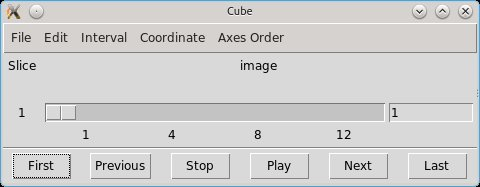
\includegraphics{mecube_raw.jpeg}
\caption[Example of DS9 cube diaglog box]{This is an example of the cube box that will open when you load a raw image in DS9.}
\label{fig:mecube}
\end{figure}

\begin{figure}[h]
\centering
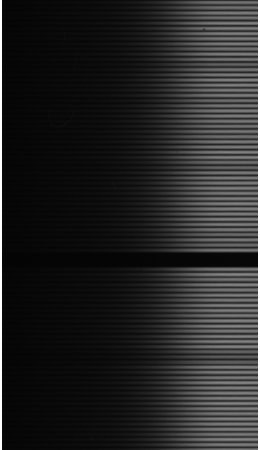
\includegraphics{raw_flat.jpeg}
\caption[Example of DS9 cube diaglog box]{This is an example raw image. Specifically this is a flat image, but you can also open the raw science and arcs. Each row you see is a fiber, and in the x direction is wavelength.}
\label{fig:rawflat}
\end{figure}

\subsection{What is an MDF?}
The mask definition file (MDF) stores information about the IFU and is ``attached'' to the raw images as one of the first steps in the data reduction process. The actual file is in binary fits format and comes with the Gemini IRAF package. The files are called either ``gsifu\_slitr\_mdf.fits'' or ``gsifu\_slits\_mdf.fits'' for the 1- and 2-slit data, respectively, and can be found in your IRAF/Gemini folder (probably a directory path similar to \ty{$\sim$/iraf/gemini/gmos/data/}) or by typing \ty{cd gmos\$data} in the IRAF/PyRAF environment. Reading the file into Python (example below) as a fits table reveals all the table columns: the fiber number (column name ``NO''), x and y spatial position of each fiber in both arcseconds (``XINST"/``YINST") and pixels (``XLDIS"/``YLDIS"), which block (bundles of 50 fibers) that the fiber is in (``BLOCK"), and whether the fiber is good or bad (``BEAM"). 

\autoref{figure:1} shows the spatial positions of the fibers over an example galaxy on the top, while the bottom image shows the 2D information that is recorded on the CCD (wavelength on the x axis and fiber number on the y axis). This illustrates why we need the MDF to map the 2D image we get from the CCD to a 3D data cube of x and y position and wavelength later in the reduction.

The ``BEAM'' column tells us which fibers are good and bad (good fibers will have BEAM=1 while bad will have BEAM=-1). See \autoref{fig:bad} for an example of what good/bad fibers look like and see \autoref{badfiber} for an example of why you may need to use/change this information. 

\chapter{Setting Up Your Workspace}

There are some things you'll need to install (or update) before using this pipeline. The author highly recommends working in the Ureka environment, which includes easy-to-install versions of IRAF, Python, and PyRAF. Since this code is written for PyRAF, Ureka is indeed quite handy. Instructions on how to download Ureka can be found here: \url{http://ssb.stsci.edu/ureka/}. This pipeline was written and test using Ureka version 1.5.1 on cielo. Follow the instructions for making IRAF, and check your login screen to make sure it says you're using IRAF 2.16:

\begin{verbatim}
> pyraf

NOAO/IRAF PC-IRAF Revision 2.16 EXPORT Thu May 24 15:41:17 MST 2012
  This is the EXPORT version of IRAF V2.16 supporting PC systems.
\end{verbatim}

There is also an updated IRAF Gemini package you'll want to install. This version is not included in the Ureka download, but includes some updated tasks you will be using. Here's the link to this newest version as of February 2016: \url{https://www.gemini.edu/?q=node/11823}. You'll also want to check this when you're done by loading the `gemini' package in IRAF:

\begin{verbatim}
--> gemini

     +------------------- Gemini IRAF Package -------------------+
     |             Version 1.13.1, December 7, 2015              |
     |             Requires IRAF v2.14.1 or greater              |
     |              Tested with Ureka IRAF v2.16                 |
     |             Gemini Observatory, Hilo, Hawaii              |
     |    Please use the help desk for submission of questions   |
     |  http://www.gemini.edu/sciops/helpdesk/helpdeskIndex.html |
     +-----------------------------------------------------------+
\end{verbatim}

This pipeline also makes use of a PyRAF script called PyFU which was written by James Turner, a support scientist at Gemini. The code will align and sum the data cubes we make during the reduction process. The package is available at the Gemini Data Reduction Forum (\url{http://drforum.gemini.edu/topic/pyfu-datacube-mosaicking-package/}), and comes with instructions on how to install and point to the package from your login.cl file.

You may also need to download L.A.Cosmic, an algorithm that finds and removes cosmic rays. You can read more about it at \url{http://www.astro.yale.edu/dokkum/lacosmic/}. You can download the IRAF spectroscopic version from that website, and will need to add a line in your login.cl: ``task lacos\_spec = /path/to/where/you/put/it/lacos\_spec.cl''. The pipeline will call this task during the cosmic ray removal step.

%(For future, may add Voronoi binning algorithm download, too.)
If you are new to data reduction in general, you will want to download DS9, an astronomical imaging application that you'll use to view our data as you progress through the pipeline. Download DS9 from this site: \url{http://ds9.si.edu/site/Home.html}.

You will now want to download the actual pipeline. You can access the code and this handy user guide at \url{https://github.com/emsnyder/geminiDRpipeline}. Always be on the lookout for updates in the future! You can place the code anywhere you like, but a nice folder structure would be to have individual folders for each galaxy with the pipeline code a level above. 

Next, you'll want data to actually reduce. You should have flats, arcs, science frames, and a bias image (see \autoref{bias}) before getting started. You should also have response flats from the baseline twilights and a flux calibration from the standard star data (\autoref{standard} leads you there creation of these if you don't already have them). In \autoref{files} there is more info on how to get your data and on each specific file you'll need. There should also be an observing log to inspect -- your data package from Gemini should come with one, and for RESOLVE, they are called obslog.txt or just log.txt. The author has also created an alternative line list file called ``smalllinelist.dat'' that will be helpful during the wavelength calibration steps. This can be found in the \texttt{github} folder as the pipeline.

The current Gemini data are located on cielo at \texttt{/srv/two/sheila/emsnyder/gemini/data/}. From there, the folders are divided into different semesters: either 2013B, 2014B, or 2015B. In each of these folders, the galaxy data is further divided into individual folders titled the galaxy's name. Each of these folders should contain an observation log, raw flats, arcs, and science frames. There should also be folders for the baseline standards -- usually these will be named LTT\#\#\#\# or H\#\#\#, after the stars we observed for our standard. These baselines may or may not be reduced already, and so if they are not, see \autoref{standard}. If they are, just copy the needed files (usually named \texttt{*\_resp.fits} for the response files and \texttt{sfunction\_*.fits} for the flux calibration files) into your galaxy folder before starting. There should be two -- one for both the red and blue setups. You can use the same baselines for each galaxy in that semester. There may also be a bias frame already in your galaxy folder, but if not, see \autoref{bias} for how to create one before getting started.


\chapter{Data Reduction Guide}

\section{How to Use This Guide}
The author's goals for this user guide are threefold: to make it clear what you are doing in each step, to explain why each step is important and necessary, and to demonstrate how to successfully complete each step when user interaction is needed. Also included with each step is the name of the Gemini IRAF tasks being used, although the tasks are typically ``under the hood'' of the pipeline. For a more in depth look at what is going on, typing \ty{help <name of task>} inside of PyRAF will open a detailed document with information about the task and what parameters you can change. This should make editing the task parameters in the pipeline easier, if it is ever needed.

\bigskip
\section{Entering and Exiting the Pipeline}
Here are the basic start up commands: 
\begin{enumerate}
\item cd to the directory where you put your data
\item enter the Ureka environment by typing \ty{ur\_setup} in the command line 
\item enter PyRAF by typing \ty{pyraf} in the command line
%\item open a DS9 window by typing \ty{!ds9 \&} at the prompt
\item enter the pipeline by typing \ty{execfile(`/path/to/your/code/gemreductionpipeline.py')}
\end{enumerate}

\noindent To end your session:
\begin{enumerate}
\item type \ty{CTRL-C} to exit the pipeline, if not out already
\item enter \ty{.exit} to exit PyRAF
\item use \ty{ur\_forget} to exit the Ureka environment
\end{enumerate}

\bigskip
\section{Organizing and Identifying Your Data}

\noindent The very first thing the pipeline does is ask you for the folder you are working in. Be sure to include the full path to your galaxy folder (including a trailing forward slash `/'), which can be found by typing \ty{pwd} in your PyRAF window but outside of the pipeline. The pipeline checks that you are actually working inside this folder next, and will direct you to fix this if you are not. Next, it will ask if you are using a special MDF file (see \label{badfiber} for why this may be needed). If you are, be sure to give the full path to that file, and if not, just type \ty{default}.

Next, the pipeline will look in your working folder and identify which files are there. It will print out the files it finds and whether they are arcs/flats/science/bias and which central wavelength they were observed at. It is good at this very first step to open up your raw images in DS9 to visually inspect your data files for any strange data. Also, be sure check the identifications against your observing log! Every file is identified by looking in the image headers, so problems here most likely will be missing images. If these all look correct, type \ty{1} to go on, if not, press \ty{0} which will exit the pipeline and let you figure out what's wrong/missing.

\bigskip
\section{Bias + Overscan Subtraction and Trimming of the Flats and Fiber Identification}
\label{fibers}

\noindent Gemini IRAF task used: \texttt{gfreduce} \\

\noindent This very first step can often (in the author's experience) be the most time-consuming step of the entire reduction. We use the flats not only for flat fielding the science data, but also to correctly order the fibers in the raw data. See bottom of \autoref{figure:1} -- each row is an individual fiber spectrum that must be correctly numbered, which ensures that we can successfully map our raw data to a 3D (x, y, wavelength) data cube. The IRAF task \texttt{gfreduce} has many different options, but for this very first step, we are just going to attach the MDF file, do a bias subtraction, overscan subtraction, image trimming, and fiber ID so that we may extract all the spectra. We will later re-extract the flats after performing a quantum efficiency correction, but we need to identify the fibers and ensure our MDF is correct before attaching it to other files.

\begin{figure}[h]
\centering
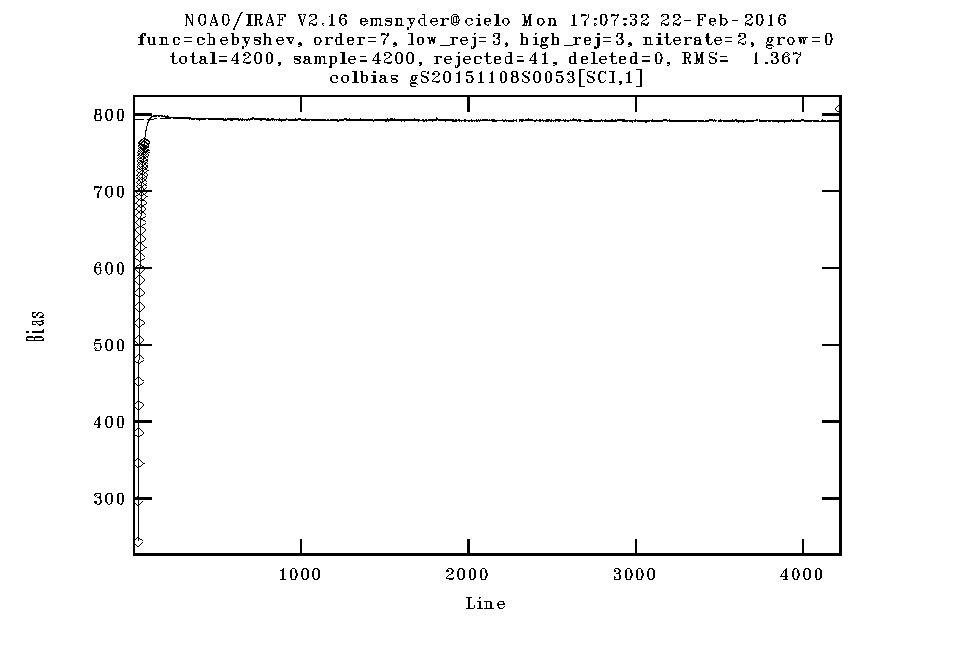
\includegraphics{overscan_example}
\caption[Overscan Subtraction Example]{An example of the overscan subtraction window that PyRAF will open during the reduction of the flats step. The solid line represents the data, while the dashed line shows the fit to that data. The diamonds are data points that are being rejected from our fit.}
\label{fig:overscan}
\end{figure}

\begin{enumerate}
\item The MDF attachment is done without user input needed. Corresponding to each input flat file, a new file is created in your working directory with the prefix `g'. A useful way to remember this could be ``g'' is for ``Get the MDF''
\item The bias and overscan subtraction and imaging trimming is mostly done without user input needed. The overscan regions are the regions of the image with no data, i.e., between the chips and amplifiers. We want to measure the count level in these regions and then trim them from our images.  Note that we also trim the outer edges of the image where there is no data in this step too, but we are not measuring the counts there for the overscan subtraction. To do this, a PyRAF window will open with the overscan level being plotted. Also plotted is a best fit line to the overscan level, and this normally looks fine as is. Press \ty{q} inside the PyRAF window to move on. There is a plot for each amplifier in the CCDs, so you will see 12 individual plots. If the fit does not look fine, you can type \ty{:order \#} and then \ty{f} inside the PyRAF window to change the order of the fit to a different number (with that number instead of \# in the previous command). Higher orders typically do better at fitting any strange features (spikes/dips). Unless something is very wrong, you probably won't need to worry about this. See \autoref{fig:overscan} for an example of what you should be seeing. This step produces a file with the prefix ``rg'', where the ``g'' comes from the previous step and the ``r'' is added for the ``subtRaction/tRimming" (this one is a stretch -- sorry).
\item Lastly, we must tackle the fiber identification. Your command window is going to ask you a few questions:
\begin{verbatim}
Extracting slit 1
Find apertures for ergS20151108S0053_1? (`yes'): 
\end{verbatim}
Here I recommend saying `yes', as usually IRAF will be able to identify the fibers correctly for you. 
\begin{verbatim}
Edit apertures for ergS20151108S0053_1? (`yes'): 
\end{verbatim}
Say `yes' to this one as well, so we can inspect the fiber IDs and make sure everything looks correct. \autoref{fig:aps} shows what this will look like -- a complete mess! But we can zoom in by typing \ty{w} in the PyRAF window, and then typing \ty{e} at the bottom-left of the first `fiber bundle' and again at its top-right. [Note: use \ty{w} and \ty{a} to un-zoom the window.] You should now have a screen that looks like \autoref{fig:aps}. I find that making this plot full-screen helps immensely. Each `bundle' contains a set of 50 fibers, which you will see numbered at the top of your screen (these are hard to see in \autoref{fig:aps}). Your job is to make sure each fiber is identified correctly -- this means no fiber is identified twice, and any bad fiber numbers are skipped (not used) in the numbering. Often I find that the low level of fiber 50 makes it get skipped in IRAF's auto-finding scheme, which makes the first fiber of the second `bundle' start at 50 instead of 51. If this happens, you can use \ty{d} in the plot window to delete the IDs for fibers 50--750, and then use \ty{m} to re-mark the fibers including the low-level fiber. This is where it can get time-consuming. \\

Figure \autoref{fig:bad} shows an example of a bad fiber not being marked in the identification process. This is exactly what we want to happen in this case. If, for example, fiber 138 was still ``on'', you would want to edit the MDF to turn it ``off" (i.e., set BEAM=-1 for that fiber number). See \autoref{badfiber} for how to do this. For the 2014-2015B slit-1 data, you will end with either fiber 742 or 743, depending on how the telescope was rotated at the time of the observation. \\

If you are pleased with your IDs, type \ty{q}. More questions will appear in the terminal, but it will want your answer inside the PyRAF graphics window.

\begin{verbatim}
Trace apertures for ergS20151108S0053_1? 
\end{verbatim}

\ty{yes}

\begin{verbatim}
Fit traced positions for ergS20151108S0053_1 interactively?
\end{verbatim}

\ty{NO} (the capitals will tell IRAF no to all)

\begin{verbatim}
Write apertures for ergS20151108S0053_1 to database
\end{verbatim}

\ty{yes}

\begin{verbatim}
Extract aperture spectra for ergS20151108S0053_1?
\end{verbatim}

\ty{yes}

\begin{verbatim}
Review extracted spectra from ergS20151108S0053_1?
\end{verbatim}

\ty{NO} \\

If you're in the blue setup (1-slit mode), this is the end of IDing for you! If you're in the red setup (2-slit mode), you'll have to repeat this process for fibers 751--1500 (usually fibers 1493 and above are missing for this group). Once complete, IRAF will extract all the spectra and create a file with the prefix ``e'' (for ``Extracted''), so in full you should have an `ergS....fits' file in your working directory. Extracting takes out the sky spectra, reorders the science spectra, and arranges them by slit. This means our output files will go from having 12 extensions to having only one or two, depending on whether you're working with 1- or 2-slit data. Since we have two different wavelength dithers, you'll have to repeat this process for the second flat, but after that, we'll use these ``erg'' flat files to identify the fibers for the rest of the files (including the arcs and science). 

\end{enumerate}

\begin{figure}[t]
\centering
\begin{subfigure}[t]{0.49\textwidth}
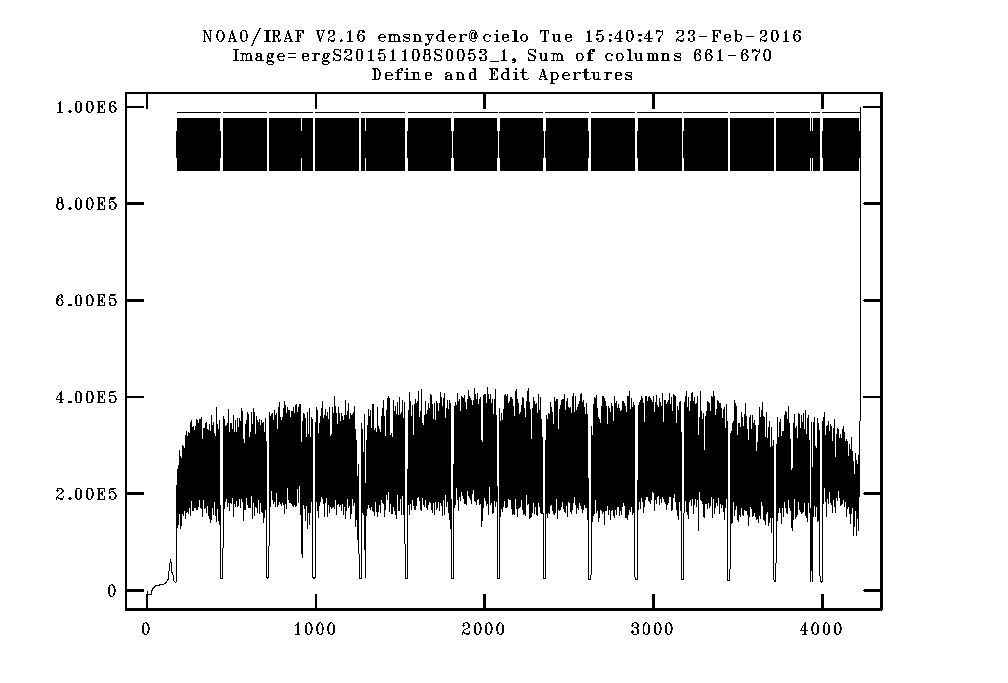
\includegraphics[width=\textwidth]{apertures1}
\end{subfigure}
\hfill
\begin{subfigure}[t]{0.49\textwidth}
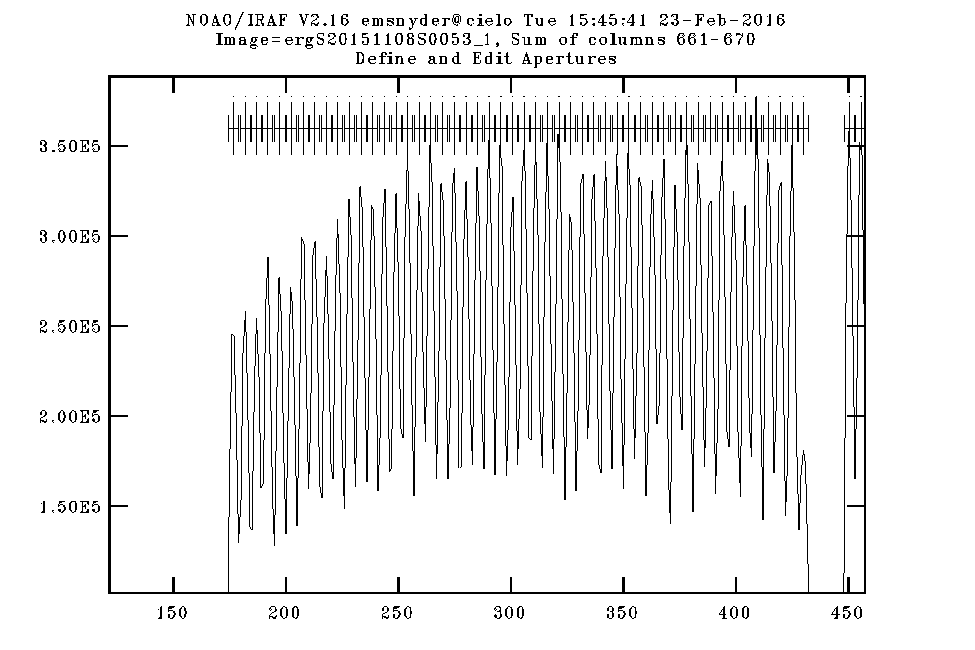
\includegraphics[width=\textwidth]{apertures2}
\end{subfigure}
\caption[Examples of the Fiber ID Step]{\textbf{(a).} A zoomed-out example of the fiber ID window that PyRAF will open during the reduction of the flats step. The numbers above each fiber are blurred together here. \textbf{(b).} An example of the fiber ID window that is zoomed-in on one set of fiber bundles. The numbers for each fiber aren't visible in this example but will be above the aperture marks at the top.}
\label{fig:aps}
\end{figure}

\begin{figure}[h]
\centering
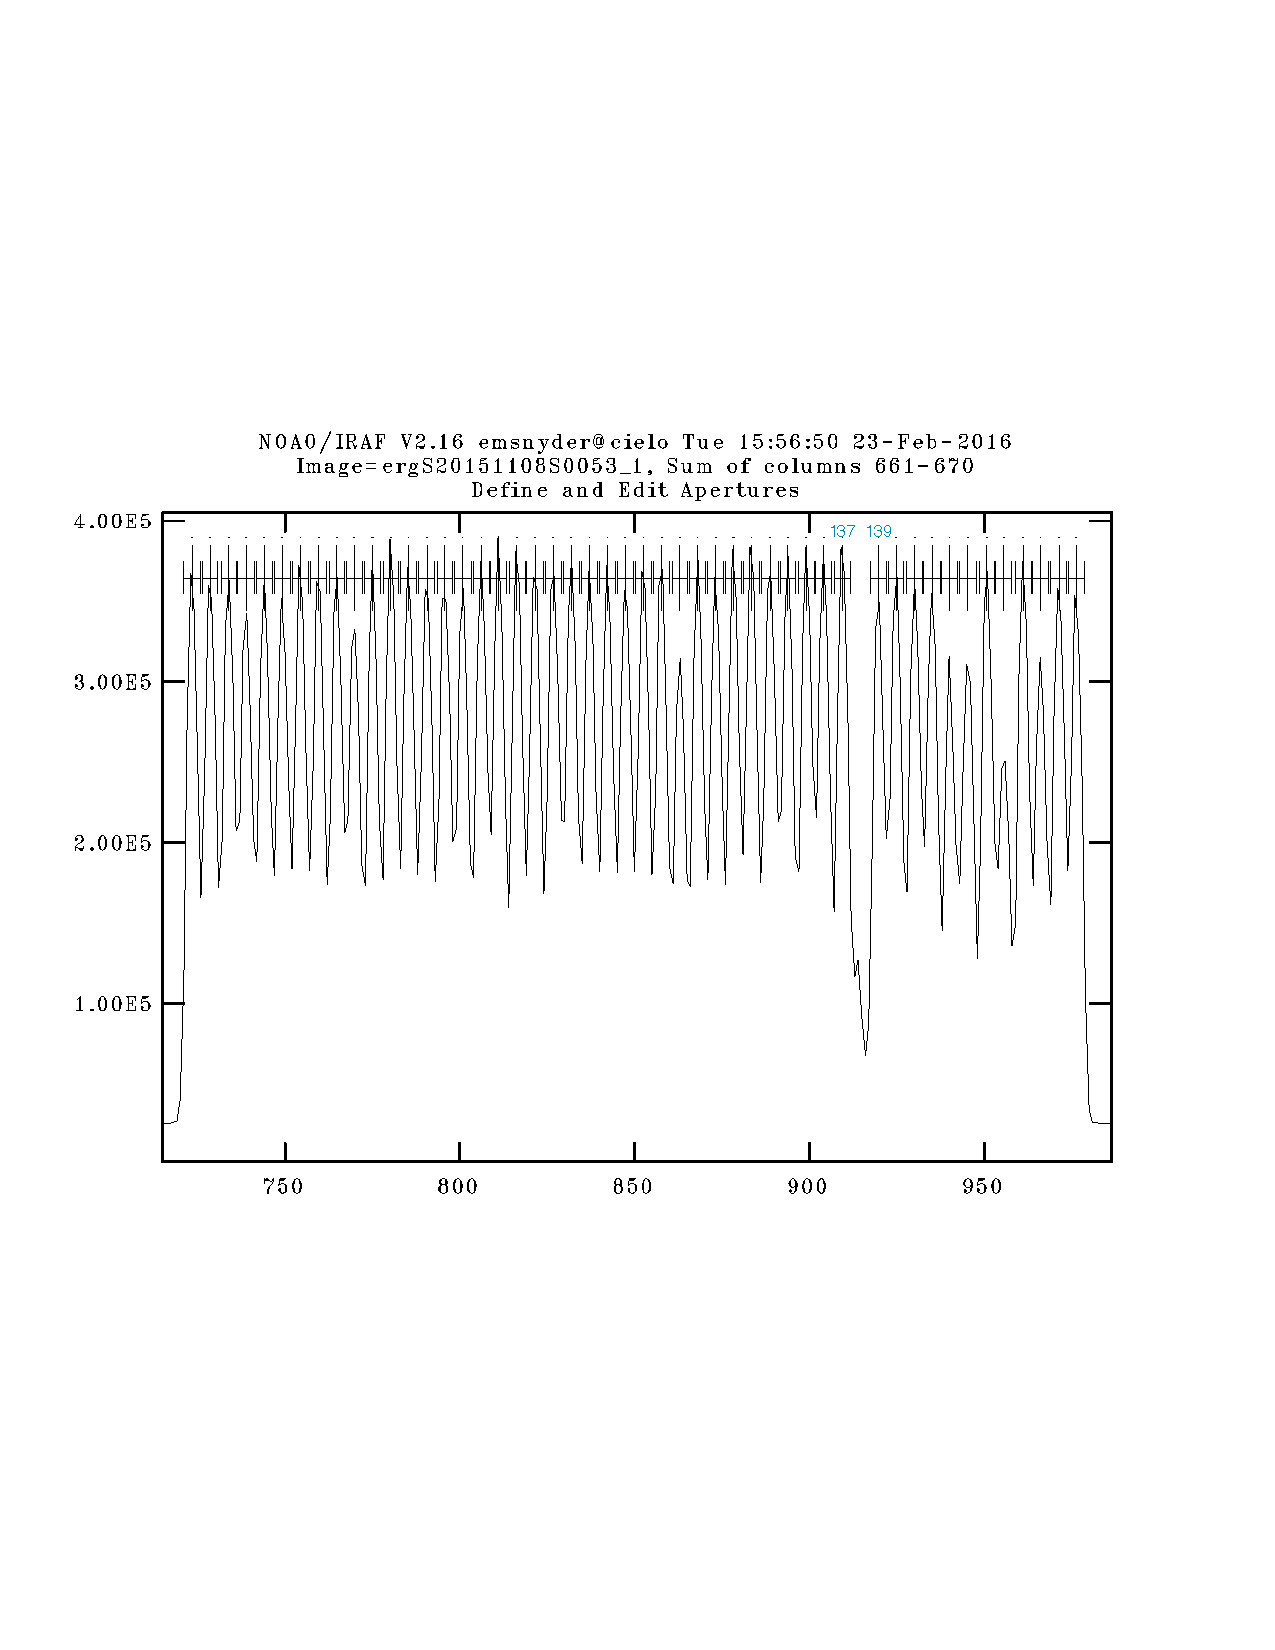
\includegraphics[scale=0.6]{badfiber_num}
\caption[Example Image of a Bad Fiber]{For this image, fiber 138 is bad. However, the MDF shows that BEAM = -1 for this fiber number, and thus that number is skipped during the identification routine.}
\label{fig:bad}
\end{figure}

\bigskip
\section{Overscan Subtraction and Trimming of the Arcs}

\noindent Gemini IRAF task used: \texttt{gfreduce} \\

\noindent Just as for the flats, we now attach the MDF file, do an overscan subtraction, and trim the arcs. We do not perform a bias subtraction on the arcs because they are read out from the CCD faster than our other data, meaning the read noise for them will be different than what's in our bias frame. We still do the overscan subtraction as a rough estimate of the bias level to subtract and we don't worry about any bias structure, which should be irrelevant if the arc lines are strong. Therefore, there is nothing interactive for this step. New files will be created with the prefix ``rg" in your working directory (they are not yet extracted). \\

\begin{figure}[h]
\centering
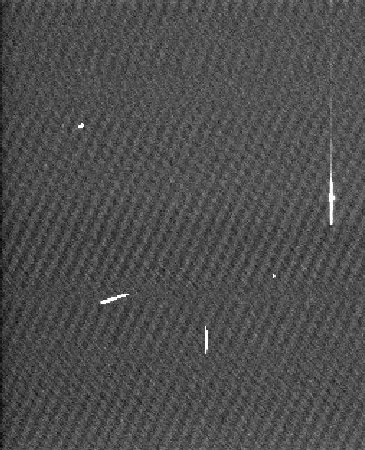
\includegraphics[scale=0.8]{CRvsBP.jpeg}
\caption[Cosmic Rays vs. Bad Pixels]{This shows you both cosmic rays and bad pixels in one of the science frames.. The long line on the right side is a bad column, whereas the other four bright spots are probably cosmic rays. These are not ``bad pixels'' because they change in every image.}
\label{fig:badpix}
\end{figure}

\bigskip
\section{Bias + Overscan Subtraction and Trimming of Science Data}

\noindent Gemini IRAF task used: \texttt{gfreduce}\\

\noindent Next, we perform the bias and overscan subtraction and trimming of the science frames. Nothing interactive is needed here, but again files will be made with the prefix ``rg''.

\bigskip
\section{Identification and Removal of Bad Pixels from the Science, Flats, and Arcs}
\label{badpix}

\noindent Gemini IRAF tasks used: \texttt{addbpm} and \texttt{gemfix}\\

%be sure to point out when revisiting that we are not doing this on the erg files!!!

\noindent Before we get too far into the reduction, we must look at one of the bias-subtracted science images and find any hot pixels or bad columns on the CCD itself that could later affect the reduction. The bad pixels are usually different for images taken with different exposure times since bleeding can occur, so we'll create a BPM for the science frames only since they have the longest exposure time. A BPM is a fits image that has the same dimensions and number of extensions as the science image, but the pixel values are only zeros and ones. The zeros denote where the pixels are good, and the ones flag where the pixels are bad. A useful caveat to bad pixels or columns on a CCD is that they will normally not change quickly, so it is okay to flag the same pixels for data sets taken in the same semester. So, if you've already created a BPM for a galaxy in the same semester, you can enter its name at the pipeline prompt to use it. If this is your first galaxy of the semester, the pipeline will lead you through how to make one.

The pipeline starts by creating an image of the correct size that's entirely made of zeros. Now, we must identify the bad pixels in our data, making note of their x and y positions and which extension they are on. The pipeline will open a DS9 window with one of the science frames. It was also open the bias image, since it is sometimes easier to see where the bad pixels are in it. The pipeline will then prompt you to look through all twelve extensions and identify any bad pixels or columns you see. If you don't see any bad pixels, you can enter \ty{0} and move on to the arcs. If you do see some bad areas, enter \ty{1}, which will bring up another prompt for you to enter the extension number, and x and y values of the bad region. The extension number can be 1-12, and x and y can extend to the full size of your image. To enter a bad rectangle, you can say x = 132:140 and y = 444:450. For a full column, you can enter * for y.

It is important to discern between cosmic rays and bad pixels/columns too. The author usually finds that cosmic rays will be curved and erratic looking, while actual bad columns will be in straight lines and may be much larger, although the extent varies so single hot pixels are also possible. See \autoref{badpix} for an example. Generally, you'll have the same bad areas in all of your images, but the extent of the damage due to these pixels can vary due to exposure time. So, if you're unsure of bad pixels vs. a cosmic ray, look in the other images to see if there are bad pixels in the same spot. 

After feeding the pipeline the coordinates of the bad pixels, it will change the BPM values to 1 from 0 at those locations. We then use the task \texttt{addbpm} to attach the BPM to our data file, so that \texttt{gemfix} can find it and interpolate over the bad pixels. The pipeline will then use this BPM to correct the science, arc, and flat frames. 

Note that in this step we are applying this correction to the images with prefixes ``rg''. This step adds the letter ``p'' for ``fixing Pixels''.

\bigskip
\section{Extraction of the Arcs}
\noindent Gemini IRAF task used: \texttt{gfextract}\\

\noindent We now extract the spectra from the arc images using the fiber IDs that were created from the flats. There is nothing interactive to be done, but file will be made with an ``e'' in front for the extracted arc spectra (the full prefix is now ``eprg'').

\bigskip
\section{Creation of the Wavelength Solution}
\label{waves}

\noindent Gemini IRAF task used: \texttt{gswavelength}\\

\noindent Next, the pipeline calls \texttt{gswavelength} and a PyRAF window will open with an image that looks like \autoref{fig:wave}. This is a 1D spectrum of the arc lamp, which we'll use to assign a wavelength to each pixel for our science data (this is called a ``wavelength solution"). You should see that some of the emission lines are being automatically marked with a $\arrowvert$ above them.

A quick aside about the lines being automatically ID'd: if you aren't using the ``smalllinelist.dat'' that was included in the download of the pipeline or if it isn't in your working directory, the pipeline will use the default line list from Gemini, which is called \texttt{GCALcuar.dat} and is located in the \texttt{gmos\$data} directory (something similar to \texttt{$\sim$/iraf/gemini/gmos/data/} outside the PyRAF environment). The difference between these two lists is that the author has taken the strongest lines from the default list and placed them into ``smallinelist.dat''. Using this list with the strongest lines only should save you time as you perform each fit since these weak lines would most likely need to be deleted anyways. When using ``smalllinelist.dat'' you should see only $\sim 10$ lines identified automatically.

Press \ty{f} to see the fit residuals, which should look something like \autoref{fig:resids}. The number to pay attention to here is the RMS. I try to keep this under $\sim0.09$\AA, which, after some experimenting, I've found produces a good wavelength solution. To delete bad points, type \ty{d} and then press \ty{f} to refit. The RMS should update after pressing \ty{f}. You can also change the order of the fit using \ty{order: \#} and then \ty{f}. The default order is 4, which seems to work well most of the time. 

At times, especially when going from slit 1 to slit 2, the first line on the left will be misidentified. You can delete lines with \ty{d} and then re-identify them by hovering your mouse above the correct line, typing \ty{m}, and then entering the correct wavelength (see \autoref{fig:wave}). Refitting with \ty{f} should then yield a better RMS value.

\begin{figure}[h]
\centering
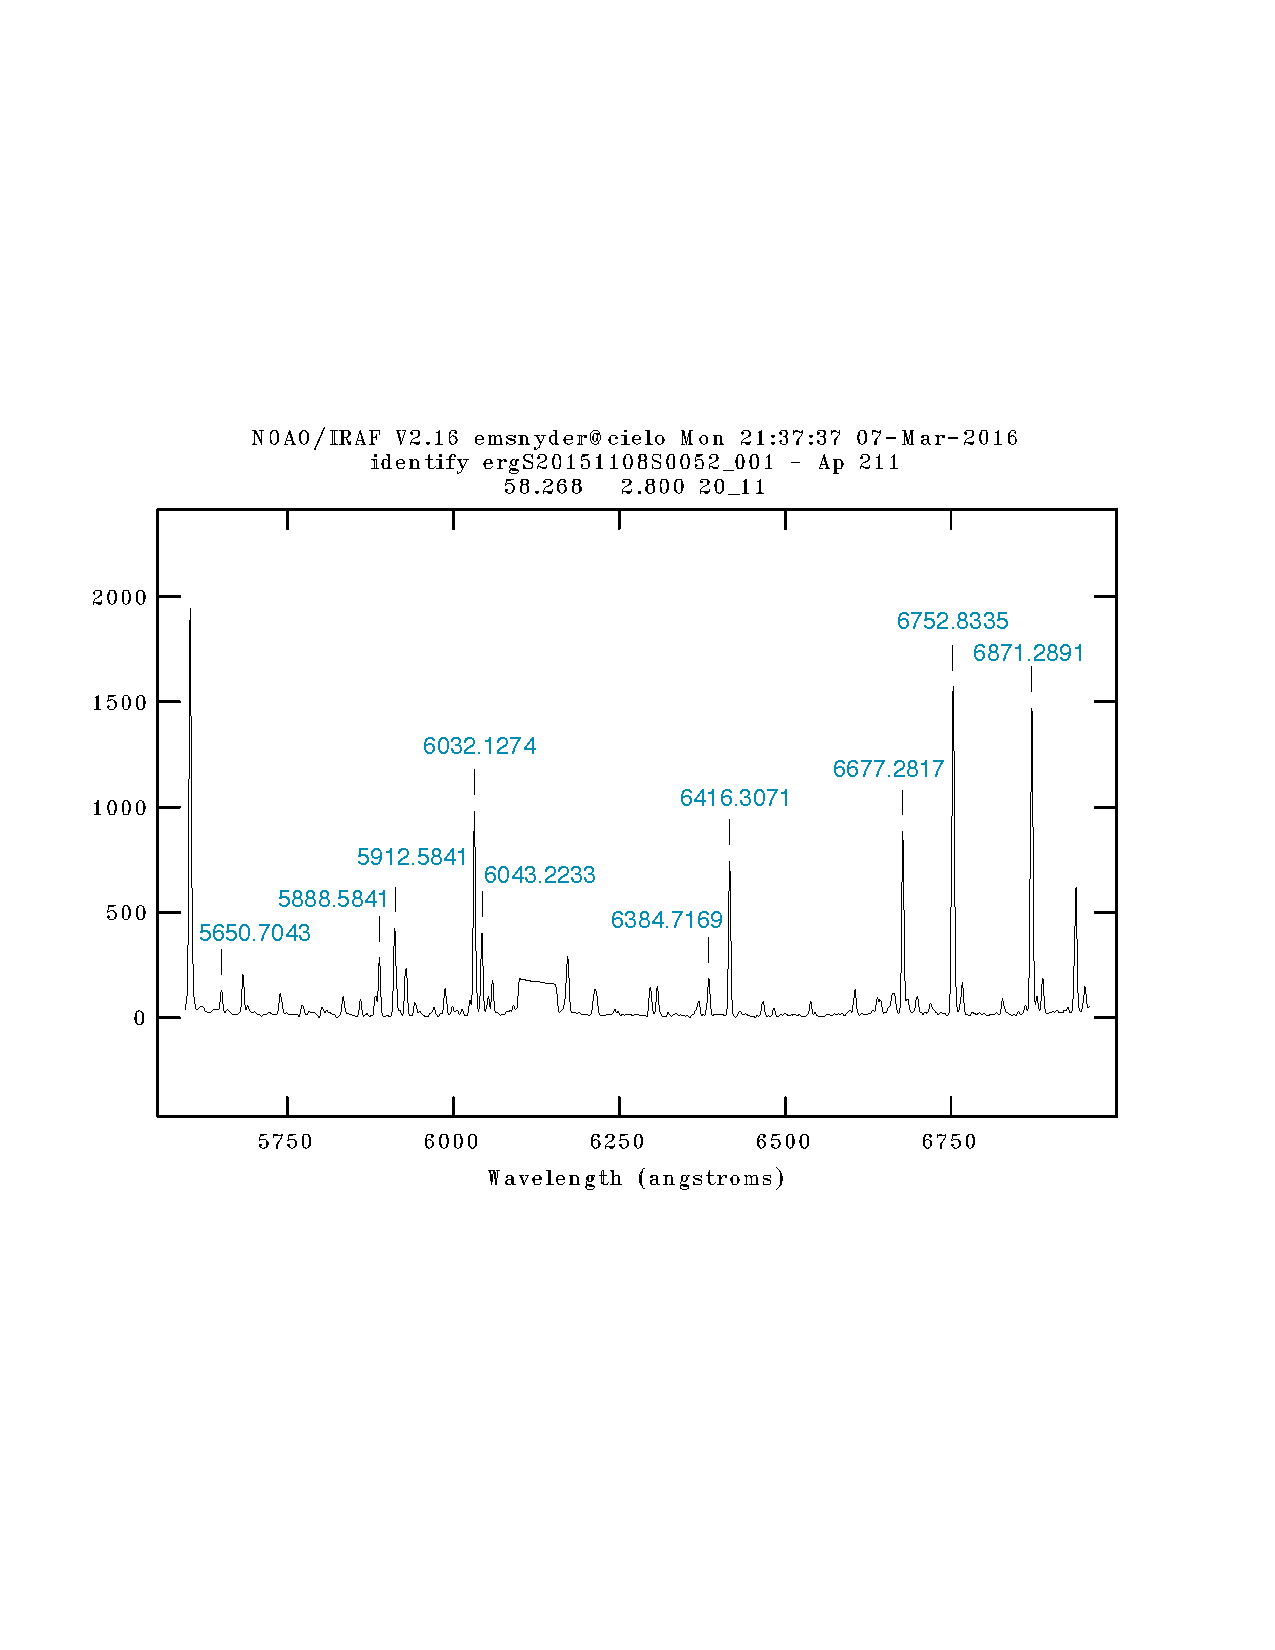
\includegraphics[scale=0.6]{wavelength_example_new}
\caption[Example of the wavelength solution]{This image shows an arc spectrum. The arc lamps have certain unchanging emission lines, by knowing the wavelengths of those lines we can create a function that assigns a wavelength to each of our image pixels.}
\label{fig:wave}
\end{figure}

\begin{figure}[h]
\centering
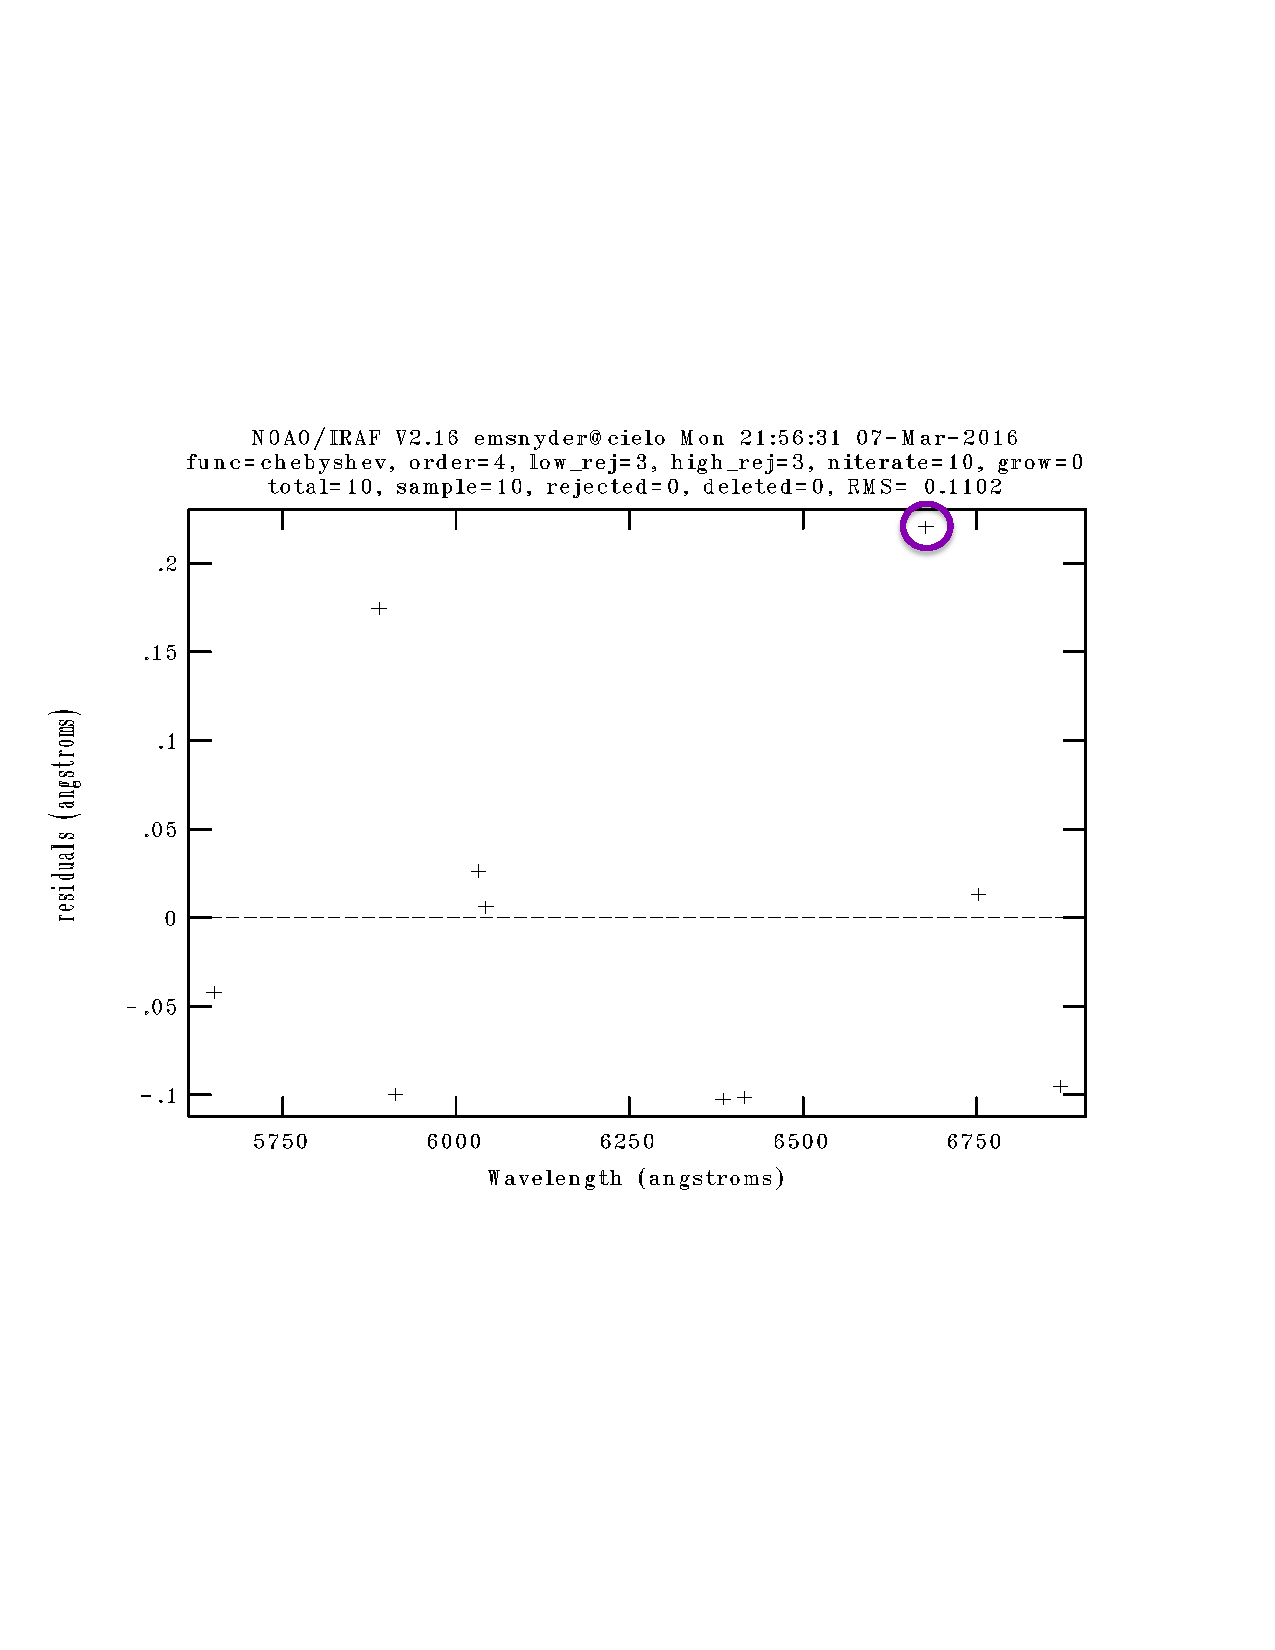
\includegraphics[scale=0.6]{wave_red_bad_new}
\caption[Example of the residuals of the wavelength fit]{This image shows the residuals of the wavelength function fit.  To improve this fit, I would delete, using \ty{d}, the circled point. You can also change the order of the fit if the default (4) doesn't fit well enough by typing \ty{order \#} and then pressing \ty{f} again.}
\label{fig:resids}
\end{figure}

You will see on your PyRAF screen some text that looks like this:

\begin{verbatim}
          Image Data    Found          Fit   Pix Shift    User Shift Z Shift      RMS
ergS20151108S0106_001 - Ap 440 10/10   10/10   -0.00557     0.00522  1.82E-6   0.0749
Fit dispersion function interactively? (no|yes|NO|YES) (`no'): 
ergS20151108S0106_001 - Ap 441 10/10   10/10    -0.0793       0.081  1.36E-5   0.0731
Fit dispersion function interactively? (no|yes|NO|YES) (`no'): 
ergS20151108S0106_001 - Ap 442 10/10   10/10    -0.0694      0.0711  1.12E-5    0.034
Fit dispersion function interactively? (no|yes|NO|YES) (`no'): 
ergS20151108S0106_001 - Ap 443 10/10   10/10   -0.00833     0.00873  9.11E-7   0.0476
Fit dispersion function interactively? (no|yes|NO|YES) (`no'): 
ergS20151108S0106_001 - Ap 444 10/10   10/10     0.0222     -0.0225  -4.0E-6     0.07
Fit dispersion function interactively? (no|yes|NO|YES) (`no'): 
ergS20151108S0106_001 - Ap 445 10/10   10/10     0.0256     -0.0259  -4.7E-6   0.0896
Fit dispersion function interactively? (no|yes|NO|YES) (`no'): 
ergS20151108S0106_001 - Ap 446 10/10   10/10      0.084     -0.0855  -1.4E-5    0.126
Fit dispersion function interactively? (no|yes|NO|YES) (`no'): yes
\end{verbatim}

My way of conquering this task is to answer \ty{no} to each prompt until I see an RMS value that needs attention. For example, the last row in the above text is where I said yes to fit the wavelength function interactively when the RMS was 0.126. If the RMS is okay, I won't fit it interactively. You will need to do this for each fiber in each arc (usually just two per galaxy). The outputs for this step are files in the database named ``idergS....\_001" and ``\_002'' (if in 2-slit mode).

\section{Application of the Calibration to the Arcs}

\noindent Gemini IRAF task used: \texttt{gftransform}\\

\noindent This step simply applies the wavelength solution you just found to the arc lamps itself. A good way to check our work here is to make sure the arc lines in the output image (which will start with the prefix ``t" for ``transformed'') are straight, as opposed to curved. See \autoref{fig:wavecal} for a before and after. If everything looks good, we can use this same solution for our science data as well. See \autoref{badwavecal} for how to correct issues or start over if needed. 

%%add example of bad wavetran!

\begin{figure}[t]
\centering
\begin{subfigure}[t]{0.49\textwidth}
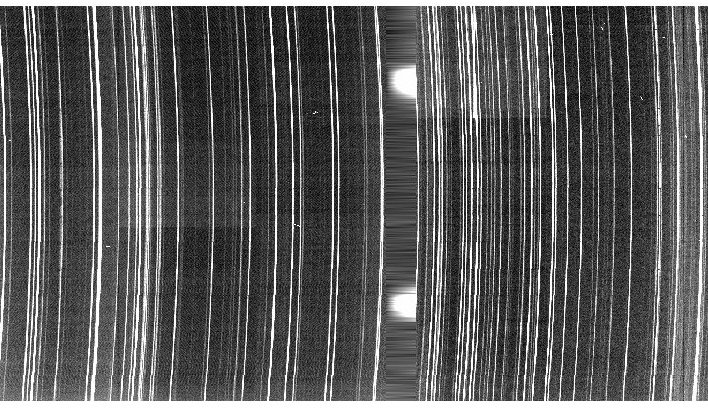
\includegraphics[width=\textwidth]{arc_before.jpeg}
\end{subfigure}
\hfill
\begin{subfigure}[t]{0.49\textwidth}
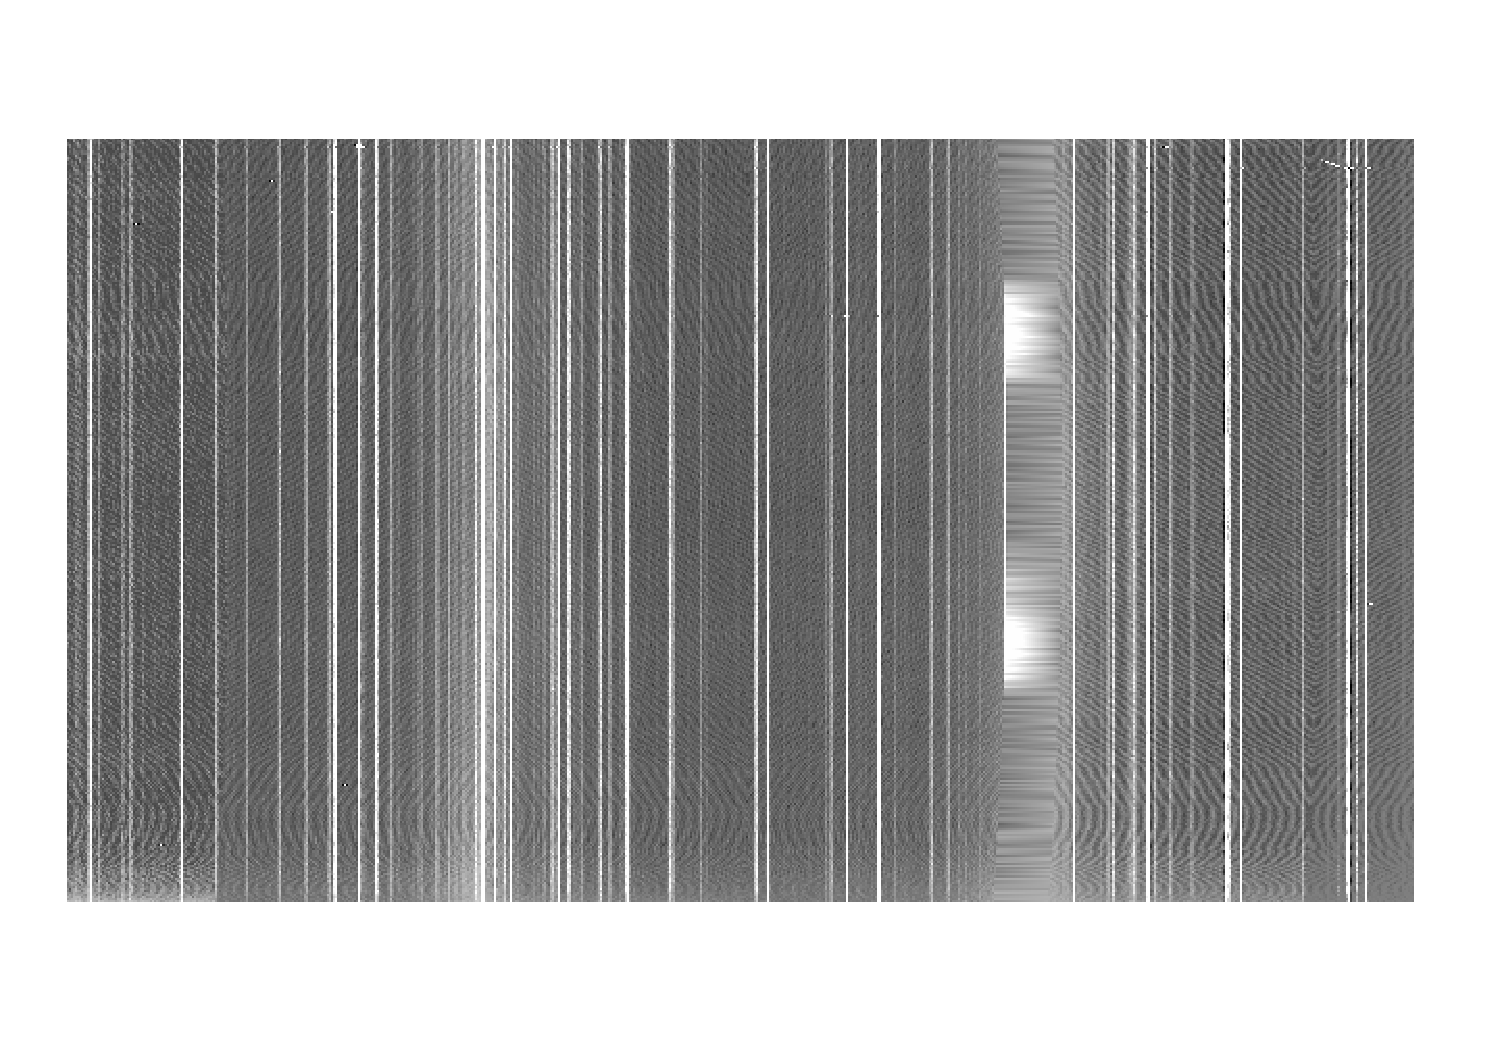
\includegraphics[width=\textwidth]{ds9}
\end{subfigure}
\caption[Before and After Wavelength Calibration]{A DS9 view of the arc \textbf{(a.)} before and \textbf{(b.)} after the wavelength transformation has been applied.}
\label{fig:wavecal}
\end{figure}

\bigskip
\section{Quantum Efficiency Correction of Flats}
\label{qecorr}

\noindent Gemini IRAF task used: \texttt{gqecorr}\\

\noindent Some CCDs will have different quantum efficiency levels between CCD sections or amplifiers, so this step corrects for this effect. The files used for these corrections is in \ty{gmos\$data} (like the MDF) and is called \ty{gmosQEfactors.dat}. Nothing interactive is required. This step creates files with the prefix ``q'' for ``Quantum efficiency corrected''.

\bigskip
\section{Re-extraction of the Flats}
\label{finalflats}
\noindent Gemini IRAF task used: \texttt{gfextract}\\

\noindent Now the flat spectra will be re-extracted, using the same fiber IDs as before, but this time pulling out the BPM- and QE-corrected and spectra. Again, nothing interactive must be done. After this step, our flats will have the prefix `eqprg'. The flat images with prefixes ``erg'' will no longer be used from now on.

\bigskip
\section{Creation of the Response Functions}

\noindent Gemini IRAF task used: \texttt{gfresponse}\\

\noindent Next, we use the twilight flats from our baseline standard data and our newly extracted from \autoref{finalflats} to create a response function for flat fielding. This response function takes into account three difference effects: pixel-to-pixel variations in the CCD itself, the wavelength-dependent pixel efficiency (i.e., pixels being more responsive to blue light than red light), and  illumination variations (corrected using the twilight flats). There is nothing interactive for this step, and the output will be named ``eqprgS...\_resp.fits''.

\bigskip
\section{Cosmic Ray Rejection}

\noindent Gemini IRAF task used: \texttt{gemcrspec}\\

\noindent Next, we use L.A. Cosmic to find and remove cosmic rays from our science spectra. The code will iterate many times, and may take a few minutes to complete. Nothing interactive is required, and a file with the prefix ``x'' is created for ``eXpunge cosmic rays''.

\bigskip
\section{QE Correction of Science}

\noindent Gemini IRAF task used: \texttt{gqecorr}\\

\noindent We now QE correct the science frames, much like we did for the flats in \autoref{qecorr}. Again, nothing interactive is needed here, and you should have a file made with the prefixes ``qxprg".

\bigskip
\section{Flat Fielding and Extraction of Science}

\noindent Gemini IRAF task used: \texttt{gfreduce}\\

\noindent Next, we use the response functions made from the twilights to flat field our science data, and then extract it. Nothing interactive is needed here, and a file with the prefix ``e'' is made.

\bigskip
\section{Wavelength Calibration of Science}

\noindent Gemini IRAF task used: \texttt{gftransform}\\

\noindent In this step, we apply the wavelength solution we found in \autoref{waves} to the science frames. There is nothing interactive for this step, and file is created with the prefix ``t''.

\bigskip
\section{Sky Subtraction of Science}

\noindent Gemini IRAF task used: \texttt{gfskysub}\\

\noindent Now, we can pull out the spectra of the sky fibers and use them to subtract the scattered sky light from the science spectra. A PyRAF window will open that looks like the left image in \autoref{fig:skysub}. The peaks that we see are probably cosmic rays that were not well subtracted, so if you hover your mouse near the peak and type \ty{d}, we can remove these artificial peaks. You can redraw the spectra after deleting using \ty{r}. When done, you should see an image like the right frame of \autoref{fig:skysub}. A file with the prefix ``s'' is made here for ``Sky subtracted''.

\begin{figure}[t]
\centering
\begin{subfigure}[t]{0.49\textwidth}
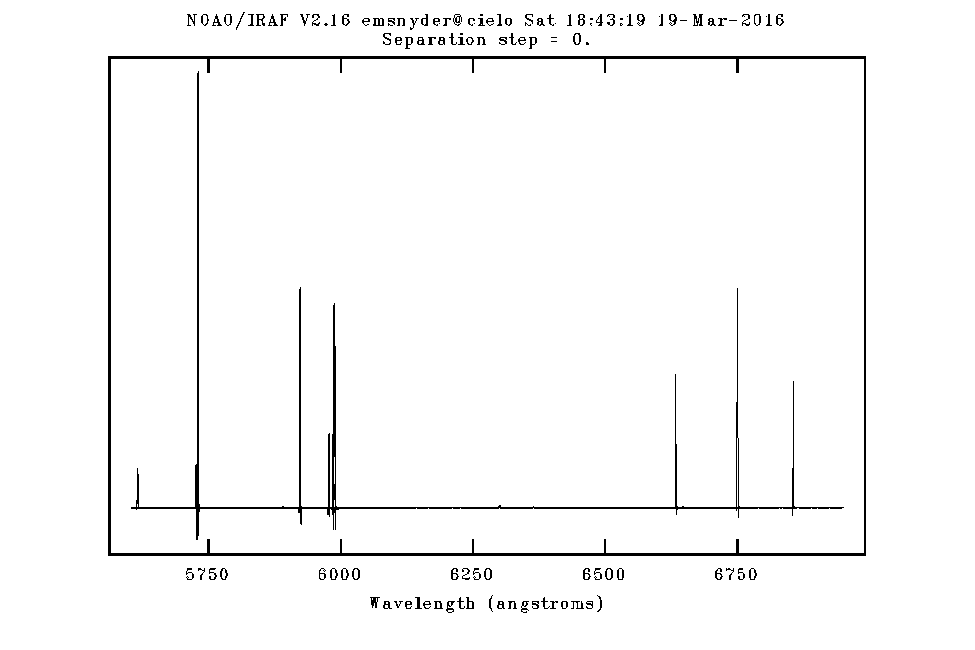
\includegraphics[width=\textwidth]{skysub_before}
\end{subfigure}
\hfill
\begin{subfigure}[t]{0.49\textwidth}
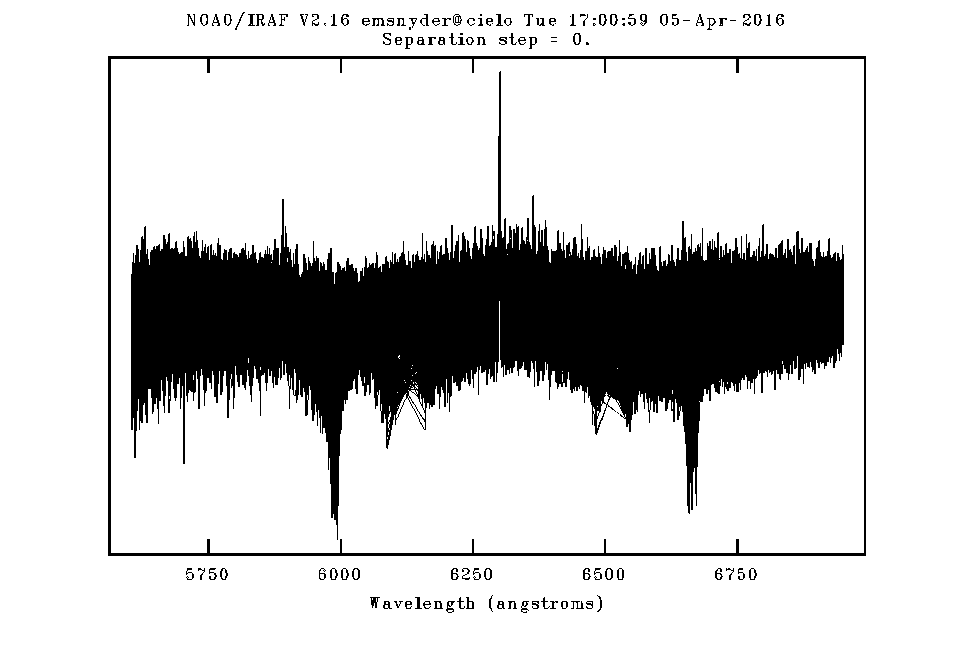
\includegraphics[width=\textwidth]{newskysubexample}
\end{subfigure}
\caption[Examples of sky subtraction]{\textbf{(a).} An example of the sky subtraction PyRAF window you'll see initially. \textbf{(b).} An example of the remaining spectra after the peaks have been deleted.}
\label{fig:skysub}
\end{figure}

\bigskip
\section{Flux Calibration of Science}

\noindent Gemini IRAF task used: \texttt{gscalibrate}\\

\noindent The second to last step of the reduction uses the flux responses from the standard star data to flux calibrate our science data. Nothing interactive is needed here, and a file with the prefix ``c" is created.

\bigskip
\section{Data Cube Creation}

\noindent Gemini IRAF task used: \texttt{gfcube}\\

\noindent Now that we're nearing the end of the reduction process, we resample our spectra into data cubes. I choose to sample the data into 0.2$''$ pixels, since that's the size of the fiber, and it will make the next step (making the WCS easier). There will be as many data cubes as there are science images. We use the task \texttt{gfcube} map the 2D images into 3D data cubes that we can later sum in the spectral direction to fill the chip gaps and increase the signal to noise ratio. If there are spatial offsets, we can use the offsets in noted in the image headers to align and sum these as well (detailed in the next steps). Files with the prefix ``d" are created here.

\bigskip
\section{Creation of a WCS Solution}

Before we can sum the data cubes, we need to assign a coordinate system to the individual cubes. To do this, we first use the information in the headers of the first extracted science file, which will have the final telescope pointing coordinate system information. In the header, there will be CRPIX1 and CRPIX2 that give the reference x and y pixels, along with CRVAL1 and CRVAL2 that are the RA and Dec values at the reference coordinates. We look inside the extracted science file for this information because we want to be able to assign an RA/Dec value to a certain fiber number. From there, we can use the spatial position of that fiber (given in our MDF) along with position angle of the galaxy observation to assign an RA/Dec to every other fiber.

A complication to this is that there an offset from the telescope pointing position to the IFU field of view. Thus, we need to correct the CRPIX1 and CRPIX2 values to reflect this small offset before assigning our coordinates. Thanks to the Gemini-South data reduction gurus James Turner and German Gimeno, we have these offsets and the pipeline can correct for this automatically. 

\bigskip
\section{Summation of the Data Cubes}

Now that the data cubes have image headers with accurate WCS coordinates, we can use the tasks included in the PyFU package to mosaic the cubes together. The Python script \texttt{pyfmosaic} looks into the headers of the supplied input data cubes and pulls out both the WCS information and the spectral offsets. It will then rebin the spectra, preserving the flux in each pixel, into one final data cube, named galaxy\_final.fits.

\chapter{Other Things You'll Want to Know}

\section{Creating the Bias Frame}
\label{bias}

Before starting the reduction, you'll want to make sure you have bias frame made, or individual biases that we can combine to make the bias frame. Each night after observing is complete, a standard set of bias frames are observed by the Gemini South operators. They are a little tricky to find in the Gemini Science Archive online database, but you can go to the ``View Associated Calibrations'' tab to find all of the biases taken for your observing program. Usually, searching on the observation date, the correct binning (CCDSUM 2 1), and the correct filter (see \autoref{table:1}) will yield 5 bias frames to download and process with the Gemini IRAF routine, \texttt{gbias}.

Outside of PyRAF, first download the frames from the database. These will come in tar file, and you can use \ty{tar -xvf gemini\_data.tar} to untar the files. The individual files are ``bzipped'' with the extension .bz2. Type \ty{bunzip2 *.bz2} to unzip the files.

Now, enter PyRAF and type \ty{gemini} and press enter, and then type \ty{gmos} and press enter again. This loads the packages needed to access the task \texttt{gbias}. Now type \ty{epar gbias} to open the PyRAF parameter editor. You should see a separate window open with \texttt{Task = GBIAS} at the top. Fill in the following boxes/checkmarks:

\begin{verbatim}
inimages = bias1.fits, bias2.fits, bias3.fits, bias4.fits, bias5.fits
outbias = <date>bias.fits
fl_over = yes
fl_trim = yes 
\end{verbatim}

\noindent Note that for \texttt{inimages} you can use wildcards, so for the biases taken on night Nov 11, you could also put \texttt{S20151111*.fits}, assuming you are working in a separate folder with no other files from that night in there. You can also name the output file (\texttt{outbias}) whatever you like, as long as it has the word ``bias'' in it. I usually name mine with the observation date followed by ``bias''.

Then press \texttt{Execute} at the top to run the task. If everything runs smoothly, you should be left with a 

\bigskip
\section{Reducing the Standard Star and Twilight Data}
\label{standard}

\bigskip
\section{When Things Go Wrong...}

\bigskip
\subsection{A Bad Fiber Identification}

\label{badfiber}
When you need to edit the MDF to ``turn off'' the number of a bad fiber during the identification step, 

To mark a fiber as bad, you can read in the appropriate fits file in IDL or Python, and change the BEAM entry for the fiber(s) of your choice. In Python, this process will probably look something like this (for the example of marking fiber 745 as bad):

\begin{verbatim}
>>> from astropy.io import fits
>>> import numpy as np
>>> hdulist = fits.open(`gsifu_slits_mdf.fits')
>>> table = hdulist[1].data
>>> table
FITS_rec(
 [(1, 0.34640503, 4.8000002, `I_1', 1, 49, 57),
  (2, 0.34640503, 4.5999999, `I_2', 1, 47, 57),
  (3, 0.34640503, 4.4000001, `I_3', 1, 45, 57), ...,
  (1498, 3.117645, 4.4000001, `A_3', 1, 45, 41),
  (1499, 3.117645, 4.5999999, `A_2', 1, 47, 41),
  (1500, 3.117645, 4.8000002, `A_1', -1, 49, 41)], 
  dtype=[(`NO', `>i4'), (`XINST', `>f4'), (`YINST', `>f4'), (`BLOCK', `S5'),
  	   (`BEAM', `>i4'), (`XLDIS', `>i4'), (`YLDIS', `>i4')])
>>> sel = np.where(table[`NO'] == 745)[0][0]
>>> sel
744
>>> table[`BEAM'][sel] = -1
>>> hdulist.writeto(`newMDF.fits')
\end{verbatim}


\noindent Once created, you can feed the file to the pipeline code as one of your first steps of the reduction process.

\bigskip
\subsection{A Bad Wavelength Solution}
\label{badwavetran}

If something looks wrong, an easy way to fix this is to delete the ID files outside of the pipeline created in the previous step along with the ``terg" files, and start again. If you're in 2-slit mode and see that only one of the slits is bad, you can delete only the bad one of these files (either ``\_001'' for the first slit and ``\_002" for the second slit), and move the other one to a temporary file name. For example, if you find slit 2 is bad for one of the arcs, you can \ty{rm} IDergS...arc1\_002, and \ty{mv} IDergS...arc2\_001 to a temporary file name. Now you can restart the pipeline, go to the wavelength calibration step, answer \ty{NO} for slit 1 and redo the fits for slit 2. There will now be two new ID files, and you can replace IDergS...arc1\_001 with your temp file.

\bigskip
\subsection{Correcting the 2014B Data with Bad Amplifier Effects}
\label{baddata}




%\end{multicols*}

%\chapter{Derivation of Kinematics}

%\section{Deriving Velocity Dispersions}
%\section{Deriving Rotation Curves}


\end{document}
